\documentclass[mathserif,serif]{beamer}
\usepackage[utf8]{inputenc}
\usepackage[english]{babel}
\usepackage{amsmath}
\usepackage{stmaryrd}
\usepackage{amsfonts}
\usepackage{amssymb}
\usepackage{hyperref}
\usepackage{graphicx}
\usepackage{url}
\usepackage{amsthm}
\usepackage{mathpartir}
\usepackage{listings}
\usetheme{Warsaw}

\lstset{
	basicstyle=\ttfamily\small,
	mathescape=false,
	frame=single,
	keywordstyle=\color{blue},
	breaklines=true
	showstringspaces=false}

\begin{document}

\newtheorem{proposition}{Proposition}
\setbeamertemplate{theorems}[numbered]

\author[Di Giacomo]
{Francesco ~Di Giacomo}
\institute[Universities Here and There] % (optional)
{
  Università Ca' Foscari di Venezia - PhD in Computer Science
}
\date{}
\title{Building Domain Specific Languages with the Metacasanova meta-compiler}

\frame{\titlepage}

\begin{frame}
	\frametitle{Introduction}
	\framesubtitle{Importance of domain specific languages}
	\begin{itemize}
		\item They allow to express the solution of a problem in a more natural way.
		\item They provide constructs that are domain-specific not provided by GPL's.
		\item They allow to develop complete application programs for a specific domain more quickly.
	\end{itemize}
	
	\pause
	\textbf{CONSEQUENCE:} It is desirable to deploy a DSL's when the scope of the application is very specific.
	
\end{frame}

\begin{frame}
	\frametitle{Introduction}
	\framesubtitle{Some DSL's examples}
	
	\begin{figure}
		\centering
		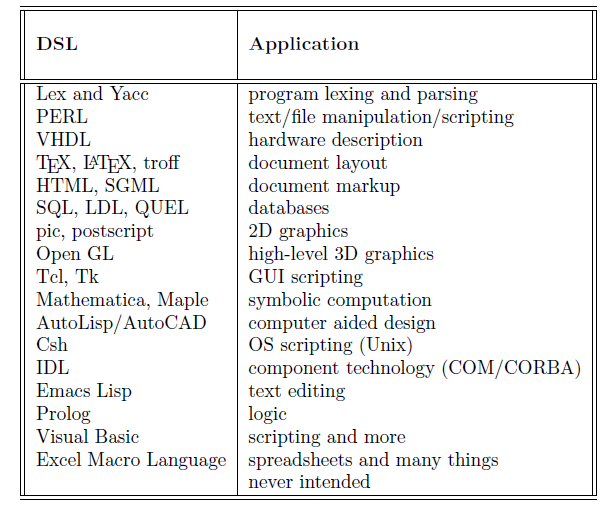
\includegraphics[scale=0.5]{Figures/dsl_table}
	\end{figure}	
\end{frame}

\begin{frame}
	\frametitle{Introduction}
	\framesubtitle{Disadvantages of DSL's}
	
	\textbf{PROBLEM}: Creating DSL's requires to implement a compiler/interpreter for the language.
	
	\begin{itemize}
		\item Compilers are complex
		\item Several modules: parser, type checker, code generator/code interpreter
		\item Require a lot of development time.
		\item Not flexible: adding features to the language compiled by hard-coded compilers takes a considerable effort.
	\end{itemize}
\end{frame}

\begin{frame}
	\frametitle{Towards meta-compilers}
	\framesubtitle{Implementing compilers is repetitive}
	
	The implementation of the compiler is a repetitive process:
	\begin{itemize}
		\item The parser can be created with parser generators (e.g. Yacc)
		\item The type system must be implemented in the host language.
		\item The operational semantics must be reflected in the generated code (code generations).
	\end{itemize}
\end{frame}

\begin{frame}
	\frametitle{Towards meta-compilers}
	\framesubtitle{Type system and semantics}
	
	How they are formalized:
	\begin{itemize}
		\item Expressed in a form that mimics logical rules.
		\item They are compact.
		\item They are readable.
	\end{itemize}
	
	How they are implemented:
	\begin{itemize}
		\item Encoded with the abstractions provided by the host language.
		\item Readability is usually lost in the translation process.
		\item The effort required for the translation is high.
	\end{itemize}
	
\end{frame}

\begin{frame}
	\frametitle{Towards meta-compilers}
	\framesubtitle{Example of semantics}
	
	Semantics of a statement that waits ford a condition or a certain amount of seconds:
	
	\vspace{0.5cm}
	\small
	\inferrule
	{\langle t - dt > 0 \rangle \; \Rightarrow \; \texttt{true}}
	{\langle \mathtt{wait} \; t;k \; dt \rangle \; \Rightarrow \; \langle \mathtt{wait} \; t - dt ; k \; dt \rangle}
	
	\inferrule
	{\langle t - dt > 0 \rangle \; \Rightarrow \; \texttt{false}}
	{\langle \mathtt{wait} \; t ; k \; dt \rangle \; \Rightarrow \; \langle k \; dt \rangle}
	
	\small
	\inferrule
	{\langle c \rangle \; \Rightarrow \; \mathtt{true}}
	{\langle \mathtt{wait} \; c;k \; dt \rangle \; \Rightarrow \; \langle k \; dt\rangle}
	
	\inferrule
	{\langle c \rangle \; \Rightarrow \; \mathtt{false}}
	{\langle \mathtt{wait} \; c;k \; dt \rangle \; \Rightarrow \; \langle \mathtt{wait} \; c;k \; dt \rangle}
\end{frame}

\begin{frame}
		\frametitle{Towards meta-compilers}
		\framesubtitle{Implementation}
		
		**STUB**
		Paste the code for wait state machine from Casanova compiler
\end{frame}

\begin{frame}
	\frametitle{Towards meta-compilers}
	\framesubtitle{Observations}
	
	\begin{itemize}
		\item Formal semantics provide a clear, compact, and simple way to describe the constructs of the language.
		\item Implementing a compiler in a GPL requires to encode the semantics within the abstractions provided by it.
		\item The result is something completely different.
	\end{itemize}
\end{frame}

\begin{frame}
	\frametitle{Towards meta-compilers}
	\framesubtitle{Idea}
	
	\large
	\color{red}
	Why not implementing a program that can take as input the language definition expressed in the fashion of the semantics rules, a program written in that language, and outputs executable code?

	\pause
	
	\vspace{1cm}
	\color{black}
	We can: this software is defined as meta-compiler.
\end{frame}

\begin{frame}
	\frametitle{Meta-casanova}
	\framesubtitle{General overview}
	
	\begin{itemize}
		\item Metacasanova is a metacompiler that uses semantics rules to define a language.
		\item A program in Meta-casanova contains:
		\begin{itemize}
			\item Data declarations
			\item Function declarations
			\item Subtypes declarations
			\item Rules
		\end{itemize}
	\end{itemize}

\end{frame}

\begin{frame}[fragile]
	\frametitle{Meta-casanova}
	\framesubtitle{Data definition example}
	
	Below the code for:
	\begin{itemize}
		\item Integer constant
		\item Sum of arithmetic expressions
		\item While loop
	\end{itemize}
	
	\begin{lstlisting}
Data "$i" -> <<int>> : Value Priority 300
Data Expr -> "+" -> Expr : Expr Priority 100
Data "while" -> Expr -> Expr : Expr Priority 10
	\end{lstlisting}
\end{frame}

\begin{frame}[fragile]
	\frametitle{Meta-casanova}
	\framesubtitle{Function definition example}
	Below the code for:
	\begin{itemize}
		\item Declaration of evaluation of expressions.
		\item Function to add a variable to the symbol table.
	\end{itemize}
	
	\begin{lstlisting}
Func "eval" -> Expr : RuntimeOp => EvaluationResult Priority 0
Func SymbolTable -> "defineVariable" -> Id : MemoryOp => SymbolTable Priority 300
	\end{lstlisting}
\end{frame}

\begin{frame}[fragile]
	\frametitle{Meta-casanova}
	\framesubtitle{Subtyping example}
	
	In the code below we declare that a value, id, and a sequence of expressions are considered expressions as well.
		\begin{lstlisting}
Value is Expr
Id is Expr
ExprList is Expr
		\end{lstlisting}
\end{frame}

\begin{frame}
	\frametitle{Meta-casanova}
	\framesubtitle{Rules}
	
	\begin{itemize}
		\item A rule is made of a set of premises and a conclusion. A premise can be a function call or a predicate.
		\item First the left part of the conclusion is evaluated. 
		\item The language does pattern matching on the function arguments and if it fails the rule is not executed.
		\item The premises are evaluated in order. The language looks for possible candidate rules for the execution, i.e. rules containing in the conclusion the function called by the premise. In case of predicates, the predicate is immediately evaluated.
		\item If the rule call fails, then the entire rule evaluation fails.
	\end{itemize}
\end{frame}

\begin{frame}
	\frametitle{Meta-casanova}
	\framesubtitle{Semantics of rule evaluation}
	
	Consider:
	\begin{itemize}
		\item A set of rules $R$.
		\item A set of function calls $F$ for each rule in $R$.
		\item A set of clauses $C$ for each rule in $R$.
		\item The notation $f^{r}$ means apply the function $f$ through the rule $r$.
		\item The notation  $\langle f^{r} \rangle$ means evaluating the application of $f$ through $r$.
		\item The result of a rule is in general a set because it is possible to allow the rule to branch, i.e. if the evaluation of a premise succeeds by using more than one rule, we return all the possible result.
	\end{itemize}
\end{frame}

\begin{frame}
	\frametitle{Meta-casanova}
	\framesubtitle{Semantics of rule evaluation}
	
	\begin{mathpar}
		\mprset{flushleft}
		\inferrule*[left=R1:]
		{C = \emptyset \\\\ F = \emptyset}
		{\langle f^{r} \rangle \Rightarrow x} \\
		
		\mprset{flushleft}
		\inferrule*[left=R2:]
		{\forall c_{i} \in C \;, \langle c_{i} \rangle \Rightarrow true \\\\
			\forall f_{j} \in F \; \exists r_{k} \in R \; | \; \langle f_{j}^{r_{k}} \rangle \Rightarrow \lbrace x_{k_{1}}, x_{k_{2}}, ..., x_{k_{m}} \rbrace}
		{\langle f^{r} \rangle \Rightarrow \lbrace x_{1}, x_{2}, ..., x_{n} \rbrace} \\
		
		\mprset{flushleft}
		\inferrule*[left=R3(a):]
		{\exists c_{i} \in C \; | \; \langle c_{i} \rangle \Rightarrow false}
		{\langle f^{r} \rangle \Rightarrow \emptyset} \\
		
		\mprset{flushleft}
		\inferrule*[left=R3(b)]
		{\forall r_{k} \in R \; \exists f_{j} \in F \; | \; \langle f_{j}^{r_{k}} \rangle \Rightarrow \emptyset}
		{\langle f^{r} \rangle \Rightarrow \emptyset}
	\end{mathpar}
\end{frame}

\begin{frame}[fragile]
	\frametitle{Meta-casanova}
	\framesubtitle{Rules - Example}
	
	\begin{lstlisting}
---------------------
eval ($i v) => ($i v)
	\end{lstlisting}
	
	\begin{itemize}
		\item The rule above does not contain premises, i.e. it is an axiom.
		\item If the pattern matching on the conclusion succeeds, i.e. the input is an integer constant, then we simply return the constant as evaluation of the expression.
	\end{itemize}

\end{frame}

\begin{frame}[fragile]
	\frametitle{Meta-casanova}
	\framesubtitle{Rules - Example}
	
		\begin{lstlisting}
eval expr1 => ($i val1)
eval expr2 => ($i val2)
<<val1 + val2>> => arithmeticResult
---------------------------------
eval expr1 + expr2 => $i arithmeticResult


	\end{lstlisting}
	
	\begin{itemize}
		\item The first rule does pattern matching on \texttt{expr1 + expr2}. This means that if the input is not in that form, the rule is not triggered.
		\item In the premises, if the result of the recursive call to the evaluation function is not an integer constant, the rule evaluation fails. This might happen when executing, for example, the sum of two strings.
		\item The third premises emits C\# code to do the sum computation.
		\item The result is another integer constant containing the sum of the two expressions.
		\item The second rule is an axiom: if the expression is an integer constant we simply return it.
	\end{itemize}

\end{frame}

\end{document}